\documentclass[11pt]{article} % use larger type; default would be 10pt

\usepackage[utf8]{inputenc} % set input encoding (not needed with XeLaTeX)

\usepackage{tikz}
\usetikzlibrary{shapes.symbols, positioning}
\begin{document}

%% -------------------------------------- CLOUD -------------------------------%%
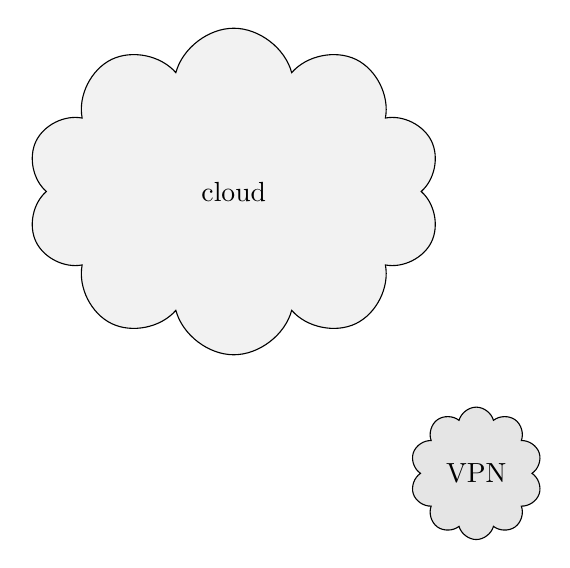
\begin{tikzpicture}

	\node[cloud, draw, fill=gray!10, aspect=1.5, inner sep=1 cm] (cloud) {cloud};
	\node[cloud, draw, fill=gray!20, below right=of cloud, yshift=-2cm] at (1.5,0) {VPN};
\path[help lines, blue!20] (0,0) grid (2,2);
\end{tikzpicture}
\end{document}